\chapter{Klassische Mechanik}

\section{Abriss der Newtonschen Mechanik}

Problemstellung der klassischen Mechanik: Orte $\vec{r}_i$ und Geschwindigkeiten $\vec{v}_i$ zur Zeit $t$ gegeben für ein System von Massenpunkten mit $1 \le i \le N$ (also $N$ Massenpunkte).

Es wirken äußere Kräfte $\vec{F}$ und Kräfte zwischen den Teilchen $i$ und $j$ ($i \neq j$): $\vec{F}_{ij}$.

Wie lauten die \textbf{kinematischen Größen} $\vec{r}_i(t)$ und $\vec{v}_i(t) = \mdotvec{r}_i(t)$ (wobei $\mdotvec{r} = \msimplediff{\vec{r}}{t}$) für beliebige Zeiten $t$ danach?

Die kinematischen Größen $\vec{r}_i(t)$ (und $\mdotvec{r}_i(t)$) werden als Lösungen gewöhnlicher Differentialgleichungen gefunden; das sind die \textbf{Bewegungsgleichungen}.

Neben diesen kinematischen Größen gibt es die wichtigen Begriffe \textbf{Kraft}, \textbf{Masse}, \textbf{Impuls} und \textbf{Energie}.


\textbf{Kraft}: vektorielle Größe, meistens $\vec{F}$ (manchmal auch $\vec{K}$); ist immer die Ursache von Bewegung oder der Änderung von Bewegungszuständen, das heißt im Umkehrschluss: kräftefrei $\rightarrow$ Bewegung unverändert 
	
Das führt auf die \textbf{Newtonschen Gesetze}: 
\begin{description}
	\item[lex prima (Galileisches Trägheitsgesetz)] es gibt Initialsysteme, in denen ein kräftefreier Körper (= Massepunkt) ruht oder sich gradlinig gleichförmig bewegt
		
	\textbf{Definition}: Jeder Massepunkt setzt der Einwirkung von Kräften einen \textbf{Trägheitswiderstand} entgegen = Masse, oder besser: \textbf{träge Masse} (Formelzeichen: $m$)
		
	\textbf{Definition}: \textbf{Impuls} $\vec{p} = m \vec{v}$
		
	\item[lex secunda (Bewegungsgesetz)] $\mdotvec{p} = \vec{F}$; meistens ist $m$ unveränderlich, dann ist $\mdotvec{v} = \msimplediff{}{t} \vec{v} = \vec{a}$ und $\vec{F} = m \vec{a}$.
		
	\item[lex tertia (actio = reactio)] $\vec{F}_{ij} = - \vec{F}_{ji}$ 
	
	\begin{figure}
		\centering
		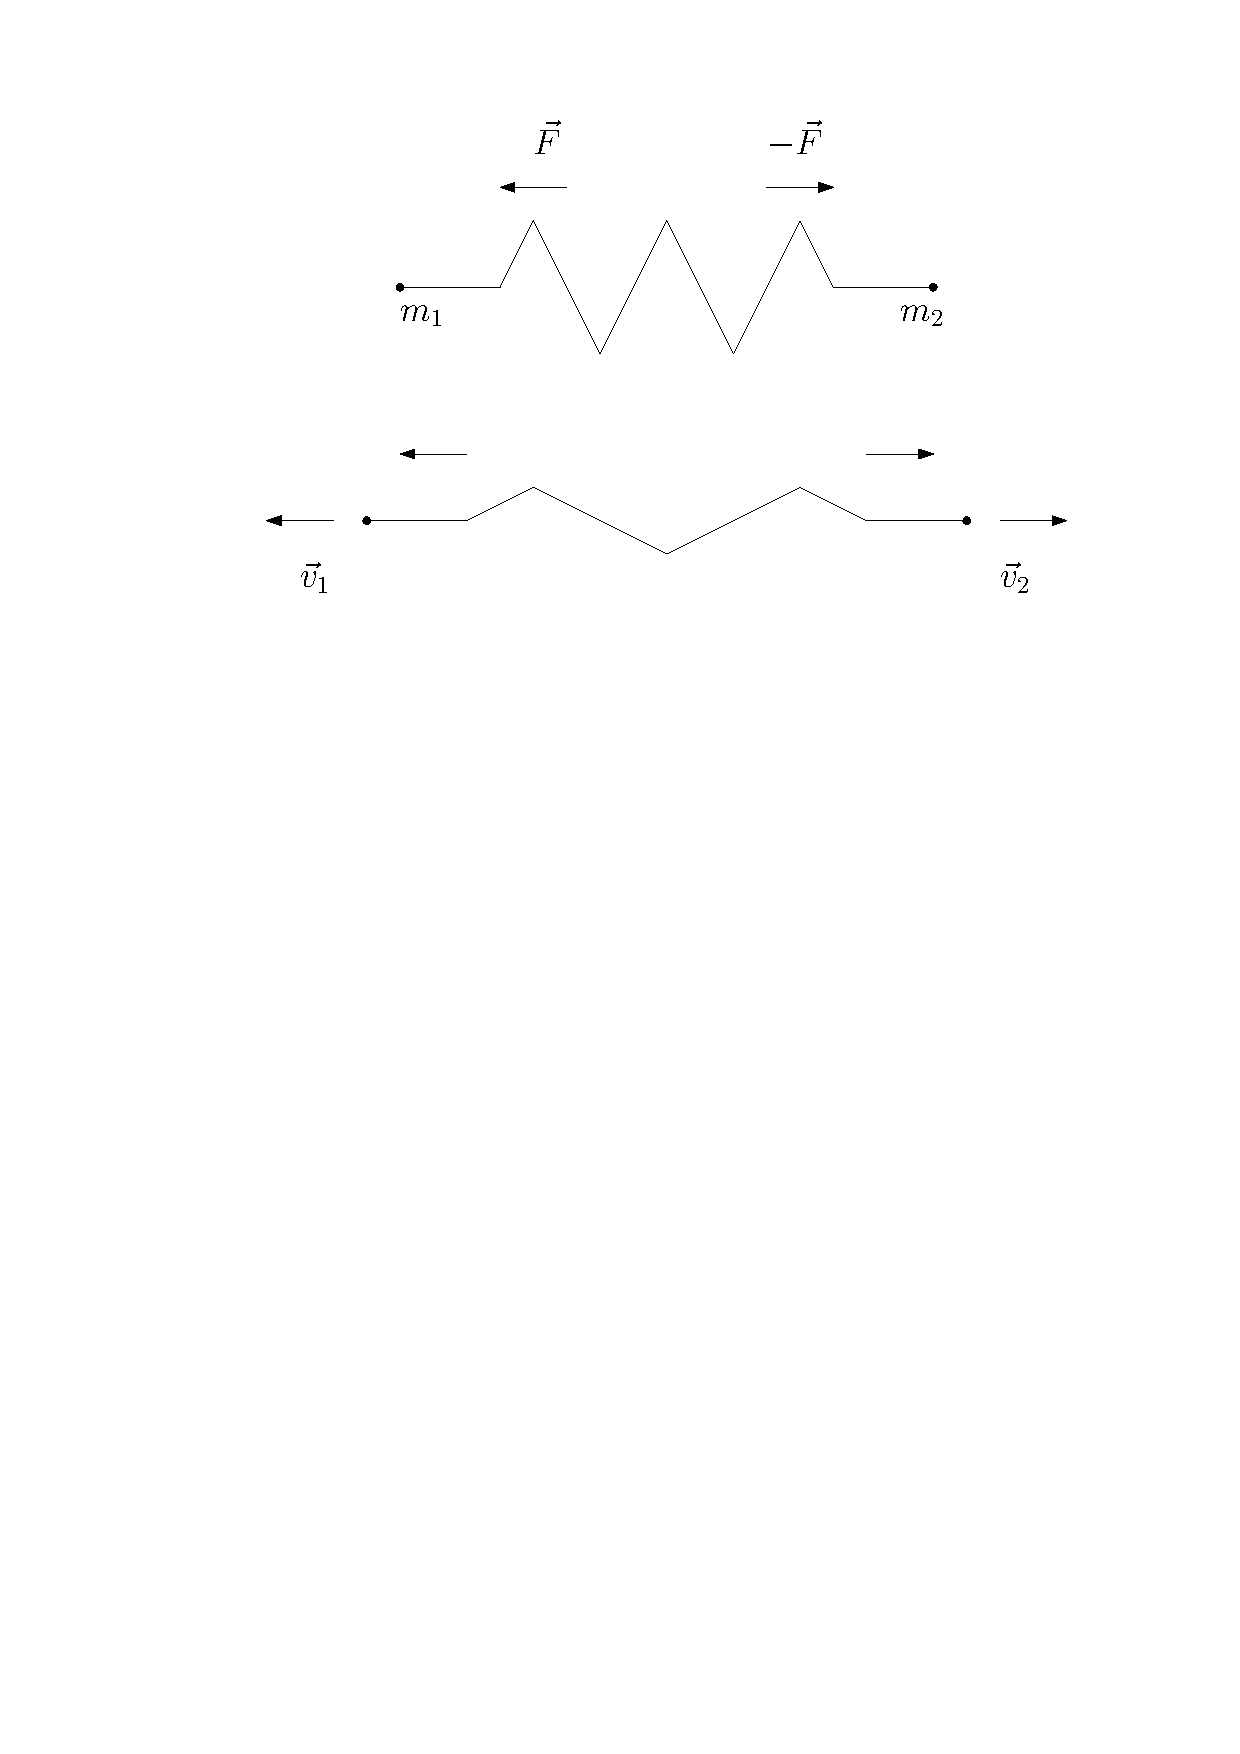
\includegraphics[scale=0.5]{figures/ch1/feder}
		\caption{actio = reactio bei einer Feder}
		\label{fig:ch1_feder}
	\end{figure}

	
	Beobachtung aus Abbildung \ref{fig:ch1_feder}: $\frac{v_1}{v_2} = \frac{m_2}{m_1}$, unabhängig von $\vec{F}$; das führt auf die Massendefinition
\end{description}

Wichtige Beispiele für Kräfte:

\begin{description}
	\item[Gravitationskraft (schwere Masse = träge Masse)] $\vec{F} = -G \frac{M m}{r^2} \hat{r}$, wobei $\hat{r} = \frac{\vec{r}}{\mabs{\vec{r}}}$ und $G$ die Gravitationskonstante ist
	
		Skizze
	
		Speziell auf der Erde: $r = r_e$, $M = M_e$, $G$
		
		Damit $F = \underbrace{G \frac{M_e}{r_e^2}}_{=: g} m = mg$ und $g \approx 9.81 m s^{-2}$; die Kraft zeigt nach unten, deswegen nur noch $F$ statt $\vec{F}$
	\item[Coloumbkraft] $\vec{F} = \frac{1}{4 \pi \epsilon_0} \frac{Q_1 Q_2}{r^2} \hat{r}$ zwischen elektrischen Ladungen $Q_1$ und $Q_2$; das sind zwei Zentralkräfte.
	\item[Lorentzkraft] $\vec{F} = e (\vec{E} + \vec{v} \times \vec{B})$: Ladung $e$, elektrisches Feld $\vec{E}$ und magnetisches Feld $\vec{B}$.
	\item[harmonischer Oszillator] lineare, stets negative (bezüglich der Bewegung) Kraft: $F = -\alpha \mabs{x}$
\end{description}

\textbf{Intertialsysteme / Nichtinertialsyseme}: In einem Inertialsystem: kräftefrei = gleichförmige Bewegung. 

Systeme $\Sigma$, $\Sigma'$ sind vollkommen gleichwertig, d.h. die physikalischen Gesetze sind forminvariant (kovariant) unter sogenannten Galilei-Transformationen. Das sind solche, die aus $\vec{r}' = \vec{r} + \vec{v}_0t$ machen, wenn sich $\Sigma$ und $\Sigma'$ mit $\vec{v}_0$ (=const) relativ zueinander bewegen. 

In \textbf{beschleunigten Systemen} gibt es sogenannte \textbf{Scheinkräfte};  zum Beispiel in rotierenden Systemen (Zentrifugalkraft, Corioliskraft).

Weitere Themen:
\begin{itemize}
	\item Schwingungsysteme (mit Dämpfung)
	\item Mehrere Massenpunkte (Eigenschwingungen)
	\item viel mehr Massenpunkte, "`starre Körper"'; Bewegung von Schwerpunkt + Rotation = "`Kreiselbewegung"'
\end{itemize}

\section{Lagrange-Mechanik}

Ausgangspunkt: Newton $m \mddotvec{r} = \vec{F}_i + \sum^N_{j \neq i} \vec{F}_{ij}$ für $i, j = 1, \dots, N$. $\vec{F}_i$ ist eine externe Kraft, $\vec{F}_{ij}$ sind Kräfte zwischen beteiligten Teilchen, paarweise. Damit: Problem vollständig formuliert, denn das sind $3N$ gewöhnliche Differentialgleichungen 2. Ordnung. Die sind im Prinzip lösbar mit den entsprechenden Anfangsbedingungen.

\textbf{Probleme}: 
\begin{itemize}
	\item Formulierung in Koordinaten $(x, y, z)_i$ ist meist zu kompliziert; damit wird die Lösung hoffnungslos.
	\item Meist Probleme mit eingeschränkter Geometrie. Zum Beispiel Perle auf kreisförmigem Draht (siehe Abbildung \ref{fig:ch1_perleaufdraht}). $(x, y, z)$ der Perle sinnvoll? $\phi$ viel geeigneter.
	\begin{figure}
		\centering
		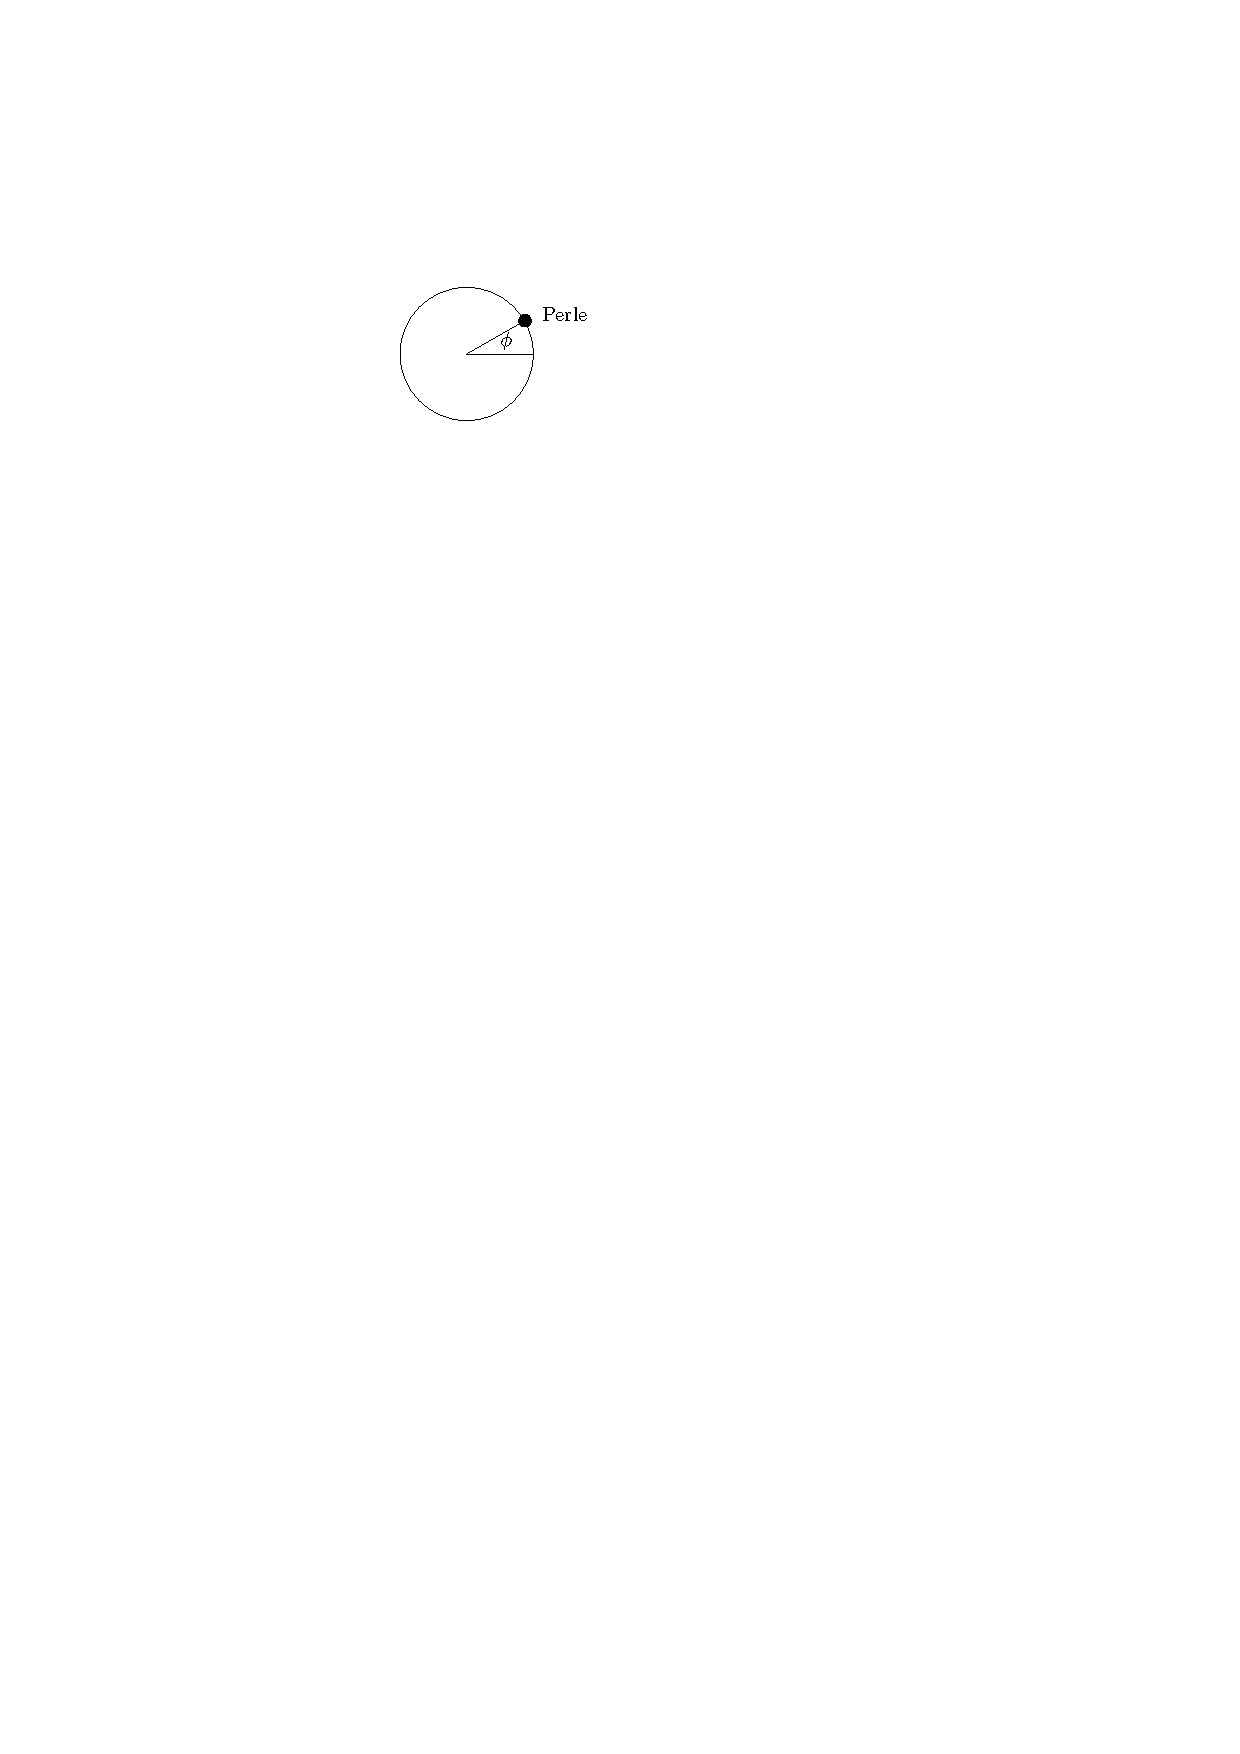
\includegraphics{figures/ch1/perleaufdraht}
		\caption{Die Position der Perle mit $\phi$ auszudrücken ist sinnvoller als mit $(x, y, z)$}
		\label{fig:ch1_perleaufdraht}
	\end{figure}
\end{itemize}

Die $\vec{F}_{ij}$ beschreiben geometrische Beziehungen auf komplizierte Weise $\rightarrow$ \textbf{Zwangskräfte} (im Beispiel die Kräfte, die die Perle auf dem Draht halten). Diese bewirken \textbf{Zwangsbedingungen}, die eigentlich direkt viel einfacher zu formulieren sind.

\textbf{Ziel der Lagrange-Mechanik}: Elimination der Zwangskräfte per verallgemeinerter Koordinaten (meist weniger als vorher)

Zwangsbedingungen sind:
\begin{itemize}
	\item A
	\begin{itemize}
		\item A1: holonom-skleronom: $\frac{\partial f_\nu}{\partial t} = 0$ mit $\nu = 1, \dots, p$ 
		\item A2: holonom-rheonom: $\frac{\partial f_\nu}{\partial t} \neq 0$ mit $\nu = 1, \dots, p$
	\end{itemize}
	\item B
	\begin{itemize}
		\item B1: als Ungleichungen $\rightarrow$ keine elimin... Bedingungen
		\item B2: differentielle Form: ???
	\end{itemize}
\end{itemize}


\textbf{Beispiele}:
\begin{itemize}
	\item Hantel (A1; siehe Abbildung \ref{fig:ch1_hantel}): $f(\vec{r}_i, \vec{r}_2) = 0$ und $(x_1 - x_2)^2 + (y_1 - y_2)^2 + (z_1 - z_2)^2 - l^2 = 0$.
	\begin{figure}
		\centering
		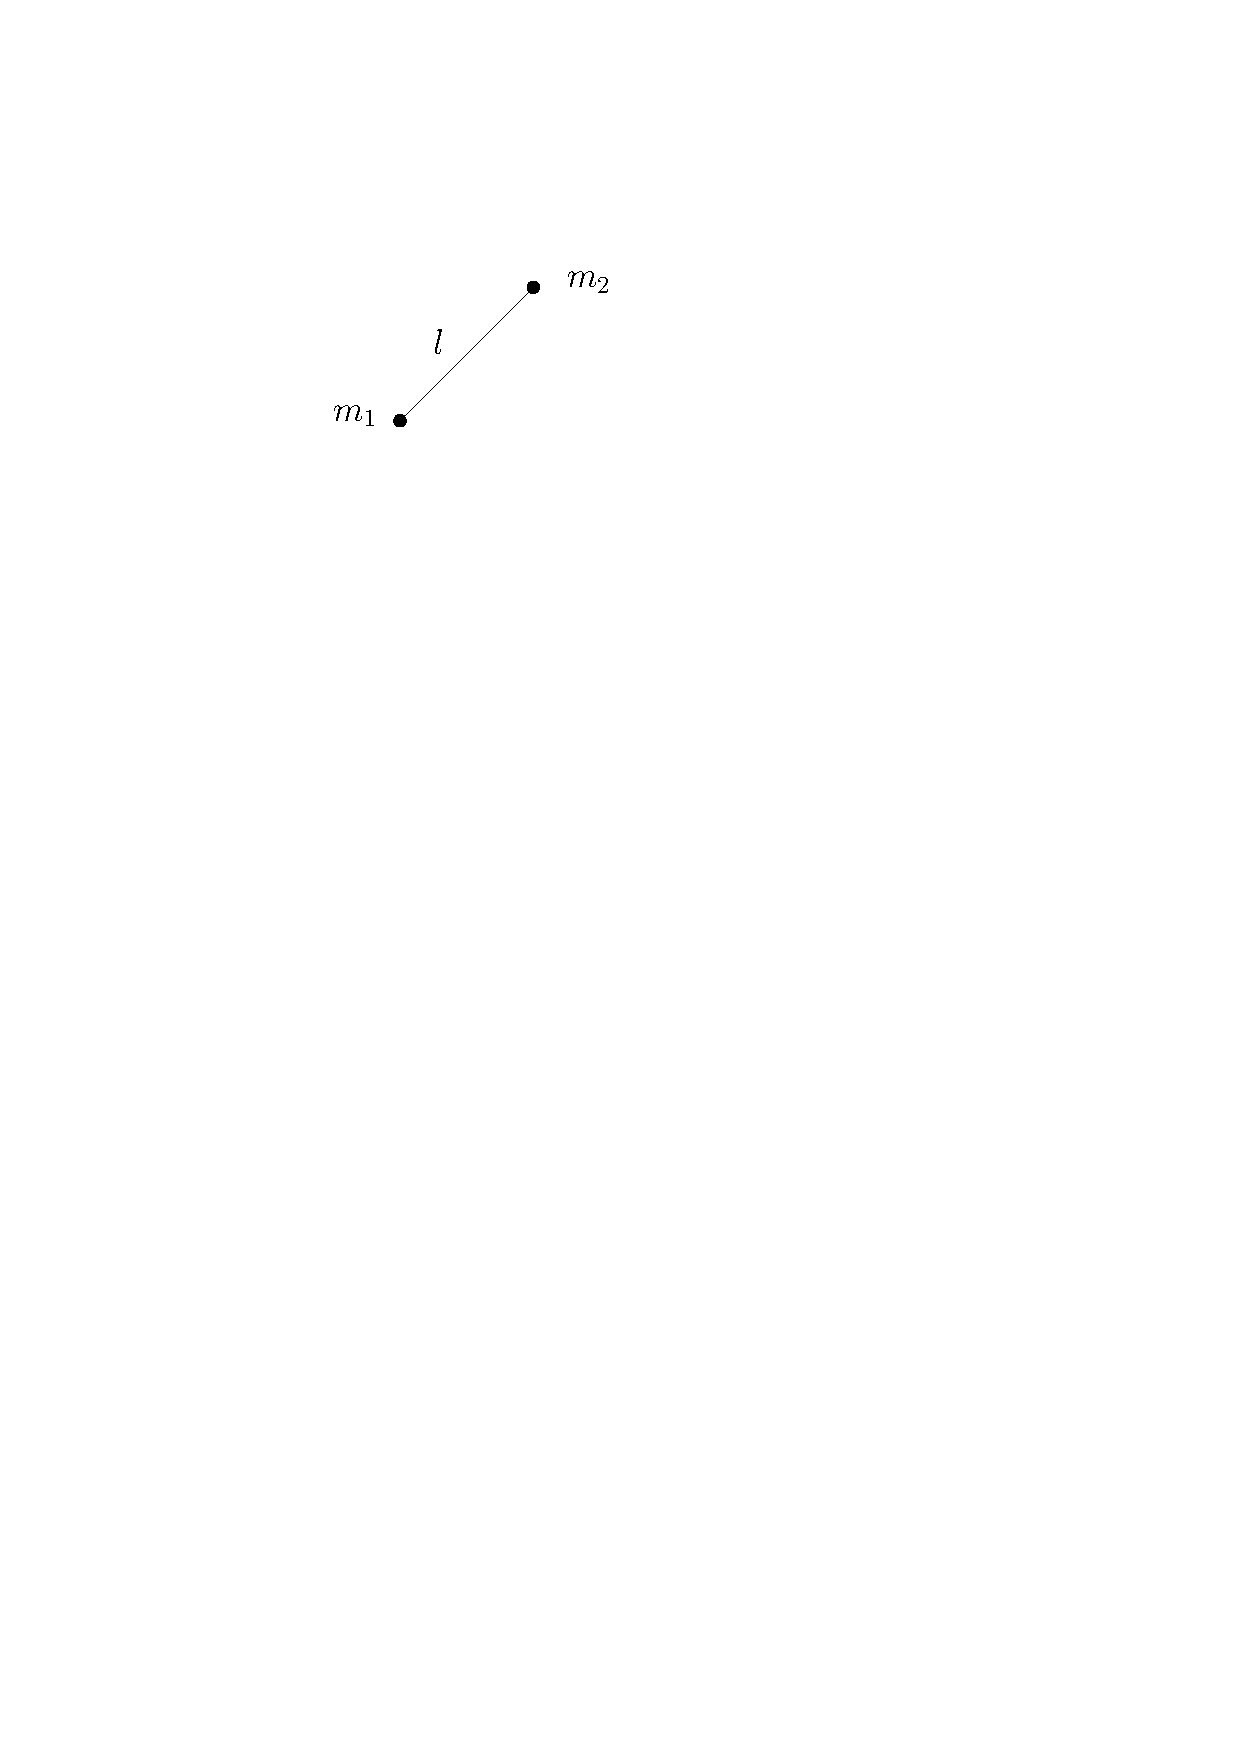
\includegraphics{figures/ch1/hantel}
		\caption{Eine Hantel der Länge $l$.}
		\label{fig:ch1_hantel}
	\end{figure}
	
	\item Ebene mit variablem Winkel (A2; siehe Abbildung \ref{fig:ch1_schiefeebene}): $\frac{z}{x} = \tan \phi(t)$
	\begin{figure}
		\centering
		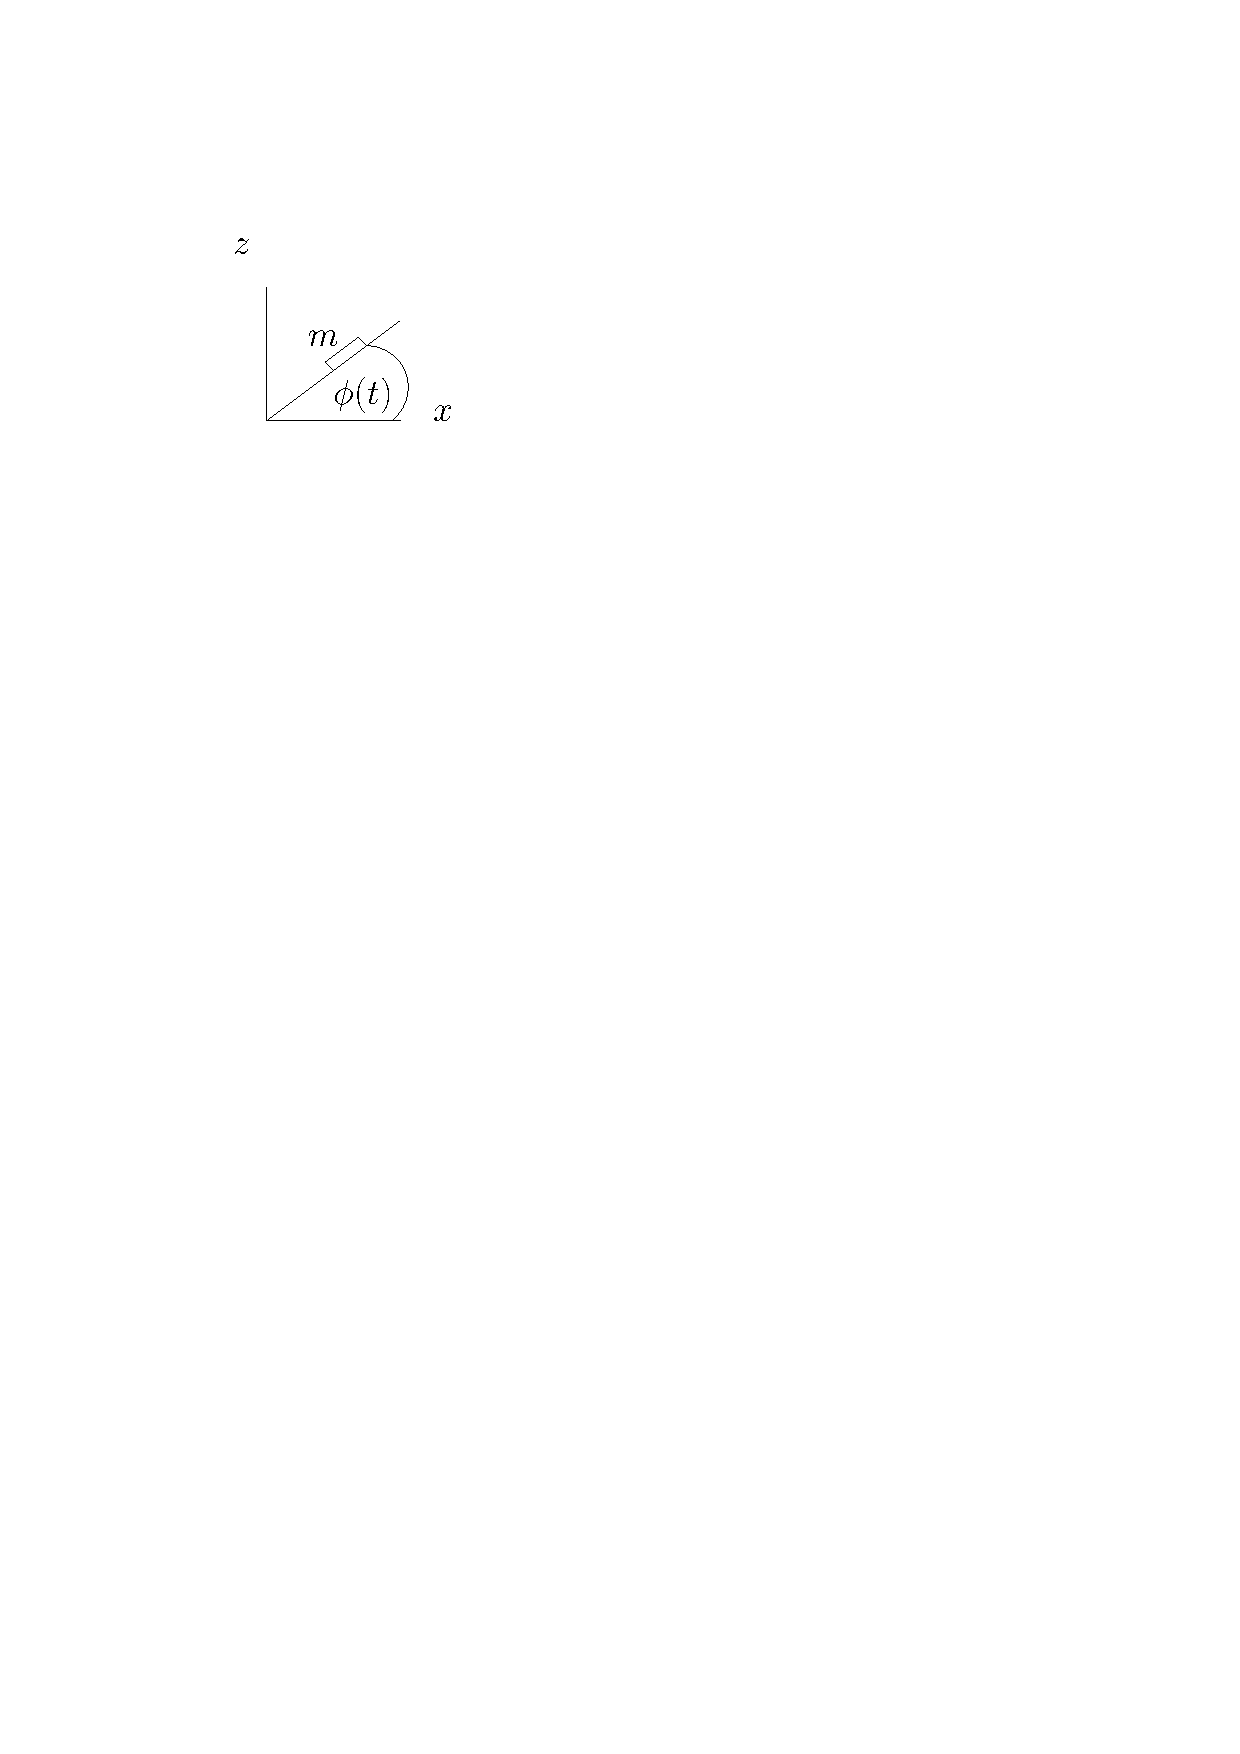
\includegraphics{figures/ch1/schiefeebene}
		\caption{Eine Hantel der Länge $l$.}
		\label{fig:ch1_schiefeebene}
	\end{figure}
\end{itemize}

Holonom: Reduktion der Freiheitsgrade $S = 3N - p$ bei $p$ holonomen Zwangsbedingungen $\rightarrow$ generalisierte Koordinaten, genannt $q_1, \dots, q_S$. Mit $\vec{r}_i = \vec{r}_i(q_1, \dots, q_S, t)$ sind Zwangsbedingungen implizit. Es gibt \textbf{keine} Beziehung $f(q_1, \dots, q_S, t) = 0$, d.h. es können keine Koordinaten eliminiert werden; $q_i$ unabhängig!

Schreibe $\vec{q} = (q_1, \dots, q_S)$ = Vektor aus dem $S$-dimensionalen Konfigurationsraum. Weiter sind $\dot{q}_1, \dots, \dot{q}_S$ die generalisierten Geschwindigkeiten.

\textbf{Bemerkung}: 
\begin{itemize}
	\item Mit $\vec{q}_0$, $\mdotvec{q}_0$ als Anfangsbedingungen sollte der Zustand zu jeder Zeit danach (oder davor) zu bestimmen sein.
	\item $\mset{q_S}$ ist nicht eindeutig, wohl aber die Anzahl $S$ (ergibt sich aus der physikalischen Problemstellung).
	\item Die $q_i$ haben eine nicht vorgegebene Dimension (müssen keine Längen sein, können z.B. auch Winkel sein). Eventuell ist die physikalische Bedeutung der $q_i$ nicht offensichtlich. Meistens sind es aber geometrische Größe.
\end{itemize}

\textbf{Beispiele}:
\begin{enumerate}
	\item Teilchen auf einer Kugeloberfläche (siehe Abbildung \ref{fig:ch1_kugel}) $\vec{r} = (x, y, z)$; $p = 1$ 
	
	\textbf{Zwangsbedingung}: $x^2 + y^2 + z^2 - R^2 = 0$, also $S = 3 - 1 = 2$. 
	
	$2$ quadratische Koordinaten, z.b. Winkel $q_1 = \nu$, $q_2 = \phi$
	\begin{figure}
		\centering
		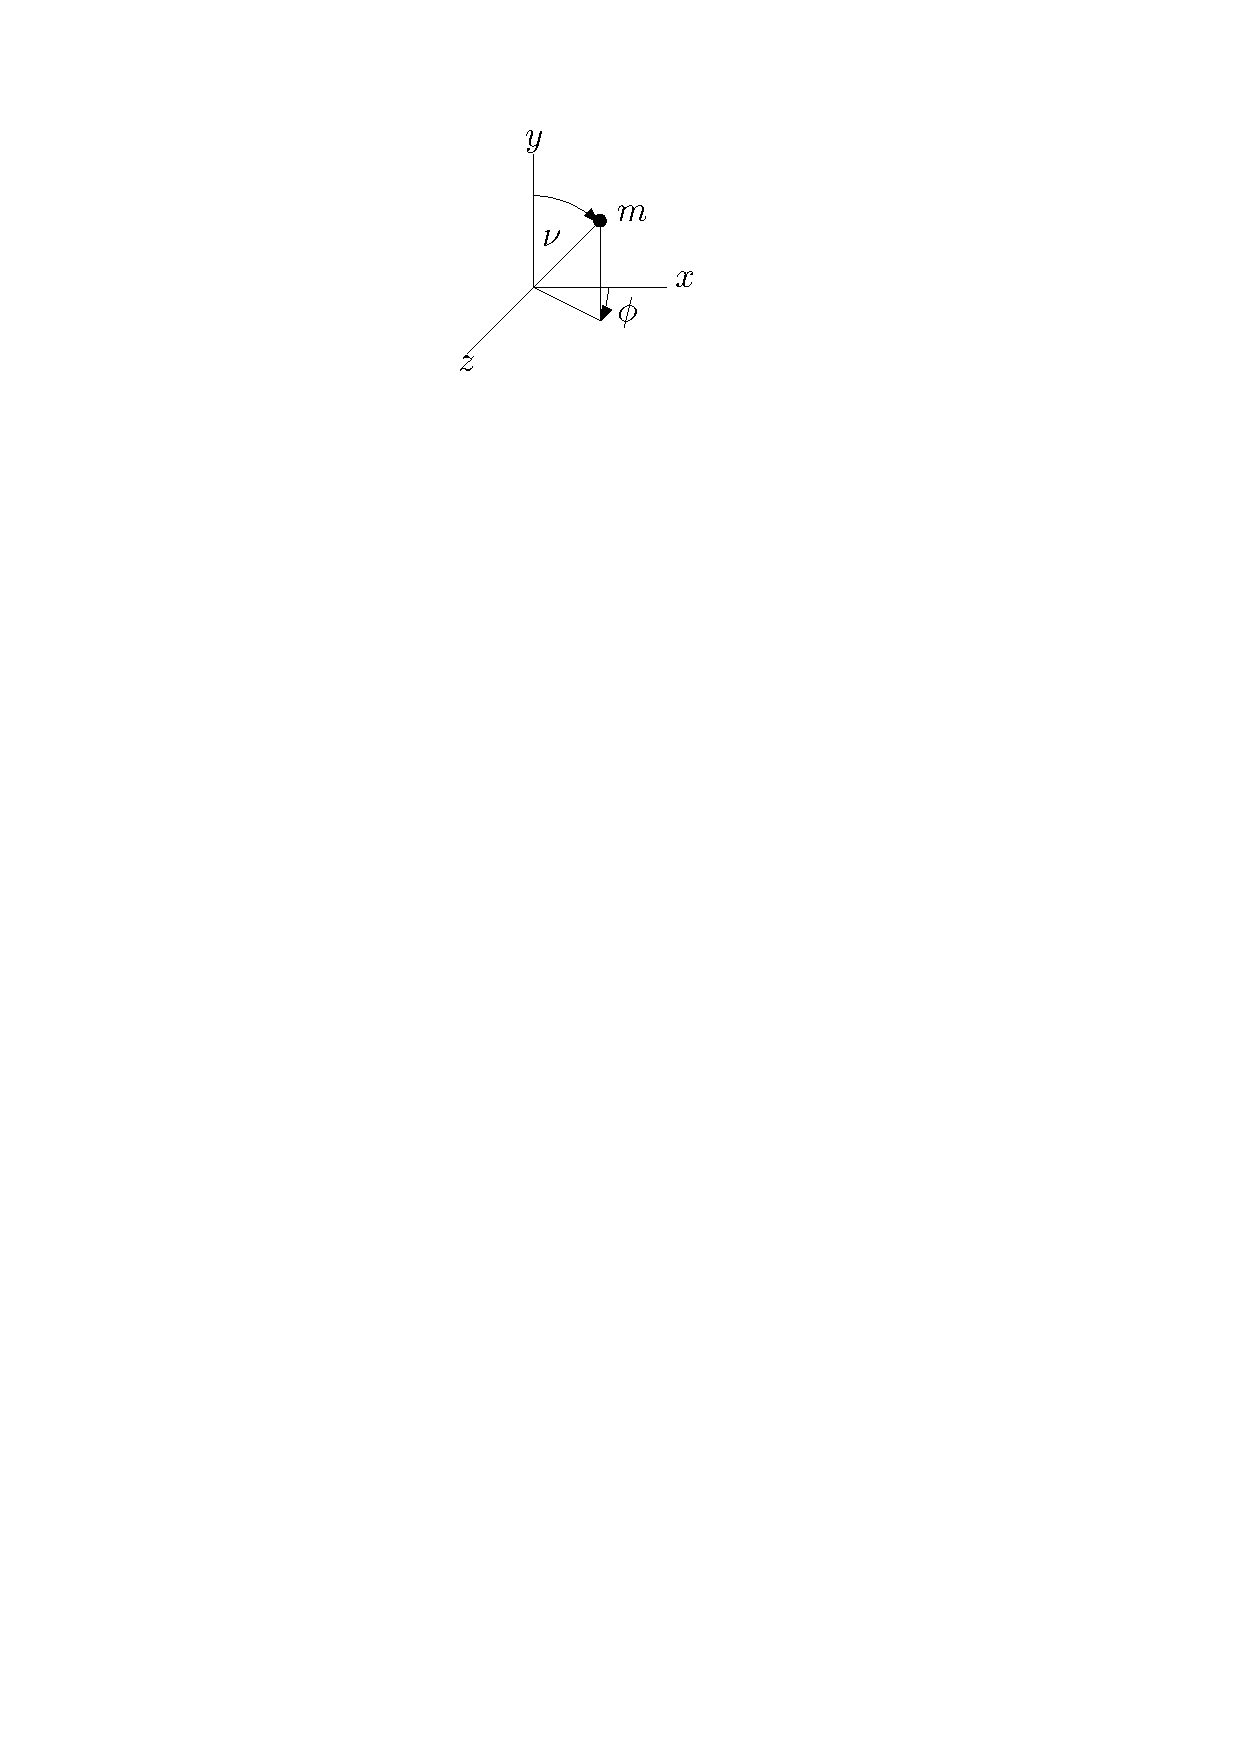
\includegraphics{figures/ch1/kugel}
		\caption{Kugel}
		\label{fig:ch1_kugel}
	\end{figure}
	
	$x = R \sin q_1 \cos q_2$, $y = R \sin q_1 \sin q_2$, $z = R \cos q_1$ $\rightarrow$ Zwangsbedingungen sind implizit, denn bei dieser Beschreibung immer erfüllt
	
	\item Doppelpendel (siehe Abbildung \ref{fig:ch1_doppelpendel}): zwei Massen $m_1$, $m_2$ = $6$ Freiheitsgrade
	
	vier davon sind holonom-shleronom: $z_1 = z_2 = ?$, $x_1^2 + y_1^2 - l_1^2 = 0$, $(x_2 - x_1)^2 + (y_2 - y_1)^2 - l_2^2 = 0$
	
	Wie viel generalisierte Koordinaten? $S = 6 - 4 = 2$ $\rightarrow$ zum Beispiel $q_1 = \nu_1$, $q_2 = \nu_2$
	
	$x_1 = l_1 \cos q_1$, $y_1 = l_1 \sin q_1$, $z_1 = 0$
	
	$x_2 = l_1 \cos q_1 + l_2 \cos q_2$, $y_2 = l_1 \sin q_1 + l_2 \sin q_2$, $z_2 = 0$
	\begin{figure}
		\centering
		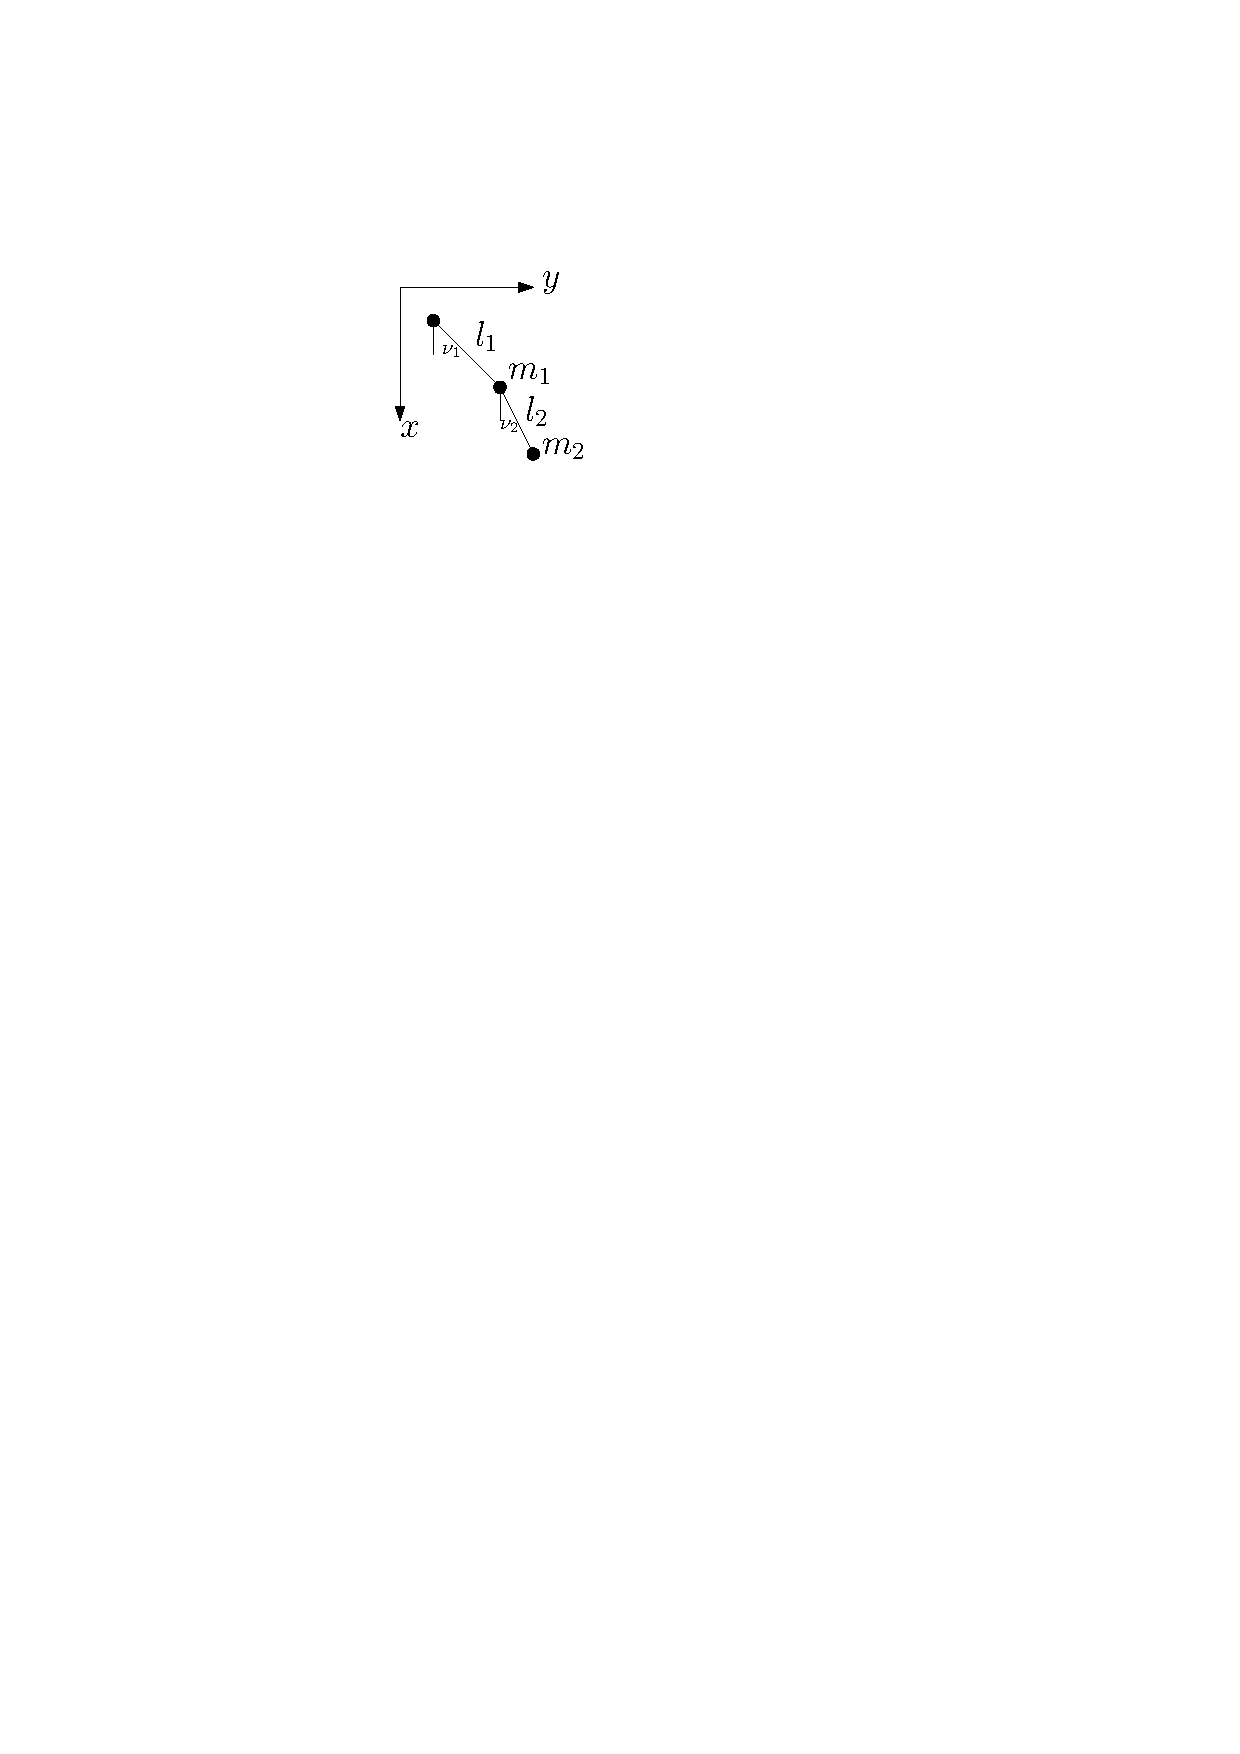
\includegraphics{figures/ch1/doppelpendel}
		\caption{Doppelpendel}
		\label{fig:ch1_doppelpendel}
	\end{figure}
\end{enumerate}

\paragraph{Virtuelle Verrückung $\delta \vec r_i$}
Eine virtuelle Verrückung ist eine willkürliche, virtuelle Koordinatenänderung, momentan ($\delta t = 0$) durchgeführt und verträglich mit Zwangsbedingungen. Hat nichts mit wirklicher Bewegung zu tun.

$\delat$ ist die virtuelle Verrückung; $d$ die tatsächliche Verrückung.


\section{Arten von Ableitungen}
\subsection{Totales Differenzial}
Betrachte $f(x_1, x_2, \ldos, x_n)$ mit $\vec x \rightarrow mathbb{R}$. Gesucht ist $df$.\\

$df = \frac{\partial f}{\partial x_1} dx_1 + \frac{\partial f}{\partial x_2} dx_2 + \ldots + \frac{\partial f}{\partial x_n} dx_n$\\

Oft: $f(x_1, \ldos, x_n, t)$
\[ \frac{dx_i}{dt} = \dot x_i \]
\[ \frac{df}{dt} = \frac{\partial f}{\partial x_i} \frac{d x_i}{d_t} + \frac{\partial f}{\partial x_2} \frac{d x_2}{d t} + \ldots + \frac{\partial f}{\partial t} = \frac{\partial f}{\partial x_1} \dot x_1 + \frac{\partial f}{\partial x_2} \dot x_2 + \frac{\partial f}{\partial x_n} \dot x_n \]